\documentclass[11pt, a4paper]{article}

% --- ESSENTIAL PACKAGES ---
\usepackage[utf8]{inputenc}
\usepackage[T1]{fontenc}
\usepackage[english]{babel}

% --- MATHEMATICS ---
\usepackage{amsmath}
\usepackage{amssymb}
\usepackage{mathtools} % For \coloneqq, etc.
\usepackage{tikz}
\usepackage{tcolorbox}

% --- LAYOUT ---
\usepackage{geometry}
\geometry{a4paper, margin=1in}

% --- HYPERLINKS ---
\usepackage{hyperref}
\hypersetup{
    colorlinks=true,
    linkcolor=blue,
    filecolor=magenta,      
    urlcolor=cyan,
    pdftitle={Handwritten MMNN 2 layer NTK computations},
    pdfauthor={Janis STG3A MMNN},
}

% --- CUSTOM COMMANDS ---
\newcommand{\E}{\mathbb{E}}
\newcommand{\dd}{\,d} % upright 'd' for integrals
\DeclareMathOperator{\ReLU}{ReLU}
\DeclareMathOperator{\Var}{Var}
\newcommand{\indic}{\mathbb{1}}

\title{Complete Summary of the Handwritten computations}
\author{Janis STG3A MMNN}
\date{\today}

\begin{document}

\maketitle

\begin{abstract}
This document recounts all the calculations, derivations, and concepts covered during my hand calculations. It covers the calculation of the expectation of products of ReLU functions applied to bivariate Gaussian variables, the application of Price's theorem, the analysis of special cases, and the study of the underlying probability laws such as the Fisher and Kibble distributions, in relation to the curse of dimensionality.
\end{abstract}
\tableofcontents
\newpage
\section{Calculating the Expectation $\E[\ReLU(X_1)\ReLU(X_2)]$}
Once we compute MMNN's NTK for 1 layer, we are left with the problem of computing the expectation $\E[\ReLU(X_1)\ReLU(X_2)]$ for a pair of random variables $(X_1, X_2)$ following a bivariate normal distribution with parameters $(\mu_1, \sigma_1, \mu_2, \sigma_2, \rho)$.

If you have 2 deterministic variables $X_1$ and $X_2$, the output of MMNN's follow a gaussian process.

Let $\sigma_1 = \|x_1\|$, where $\|\cdot\|$ denotes the Euclidean norm.
Let $\sigma_2 = \|x_2\|$, and
Let $\rho = \frac{\langle x_1, x_2 \rangle}{\|x_1\| \|x_2\|}$ be the cosine similarity between $x_1$ and $x_2$.

The covariance matrix of the gaussian process is:
\[
\Sigma = \begin{pmatrix}
\sigma_1^2 & \rho\sigma_1\sigma_2 \\
\rho\sigma_1\sigma_2 & \sigma_2^2
\end{pmatrix}
\]
The covariance matrix of the gaussian process is:
\[
\Sigma = \begin{pmatrix}
\sigma_1^2 & \rho\sigma_1\sigma_2 \\
\rho\sigma_1\sigma_2 & \sigma_2^2
\end{pmatrix}
\]




\subsection{Decomposition}
We recall the expression of mu
The approach is to standardize the variables ($Z_i = (X_i - \mu_i)/\sigma_i$) and decompose the integral into four terms:
\[
\E[\dots] = \sigma_1\sigma_2 I_{22} + \mu_1\sigma_2 I_{12} + \mu_2\sigma_1 I_{21} + \mu_1\mu_2 I_{11}
\]
where the integrals $I_{ij}$ are defined over the domain $z_1 > a$ and $z_2 > b$, with $a = -\mu_1/\sigma_1$ and $b = -\mu_2/\sigma_2$.
\begin{itemize}
    \item $I_{11} = \int_a^\infty \int_b^\infty \phi_2(z_1, z_2; \rho) \dd z_2 \dd z_1$
    \item $I_{21} = \int_a^\infty \int_b^\infty z_1 \phi_2(z_1, z_2; \rho) \dd z_2 \dd z_1$
    \item $I_{12} = \int_a^\infty \int_b^\infty z_2 \phi_2(z_1, z_2; \rho) \dd z_2 \dd z_1$
    \item $I_{22} = \int_a^\infty \int_b^\infty z_1 z_2 \phi_2(z_1, z_2; \rho) \dd z_2 \dd z_1$
\end{itemize}

\subsection{Calculation of the Components}

\subsubsection*{Calculation of $I_{11}$ (Probability)}
$I_{11}$ is the probability $P(Z_1 > a, Z_2 > b)$. It is calculated via the cumulative distribution function (CDF) of the standard bivariate normal distribution, $\Phi_2$.
\[
I_{11} = P(Z_1 > a, Z_2 > b) = P(Z_1 < -a, Z_2 < -b) = \Phi_2(-a, -b; \rho) = \Phi_2\left(\frac{\mu_1}{\sigma_1}, \frac{\mu_2}{\sigma_2}; \rho\right)
\]


\subsubsection*{Calculation of $I_{12}$ and $I_{21}$ (First-Order Moments)}

For $I_{12}$, we need to calculate:
\[
I_{12} = \int_a^\infty \int_b^\infty z_2 \phi_2(z_1, z_2; \rho) \dd z_2 \dd z_1
\]

\paragraph{Step 1: Inner integral}
We first focus on the inner integral with respect to $z_2$. The exact formula for the conditional density is:
\[
\phi_2(x,y;\rho) = \frac{1}{\sqrt{1-\rho^2}} \phi_1(y) \phi_1\left(\frac{x-\rho y}{\sqrt{1-\rho^2}}\right)
\]
Applying this formula with $x=z_1$ and $y=z_2$:
\[
\phi_2(z_1,z_2;\rho) = \frac{1}{\sqrt{1-\rho^2}} \phi_1(z_2) \phi_1\left(\frac{z_1-\rho z_2}{\sqrt{1-\rho^2}}\right)
\]
The inner integral becomes:
\[
\int_b^\infty z_2 \frac{1}{\sqrt{1-\rho^2}} \phi_1(z_2) \phi_1\left(\frac{z_1-\rho z_2}{\sqrt{1-\rho^2}}\right) \dd z_2
\]

\paragraph{Step 2: Change of variable}
Let $u = \frac{z_1-\rho z_2}{\sqrt{1-\rho^2}}$. Then:
\begin{align*}
z_2 &= \frac{z_1-u\sqrt{1-\rho^2}}{\rho} \\
\dd z_2 &= -\frac{\sqrt{1-\rho^2}}{\rho} \dd u
\end{align*}
The lower bound becomes $u_{max} = \frac{z_1-\rho b}{\sqrt{1-\rho^2}}$. The integral transforms into:
\[
\frac{1}{\sqrt{1-\rho^2}} \int_{-\infty}^{\frac{z_1-\rho b}{\sqrt{1-\rho^2}}} \left(\frac{z_1-u\sqrt{1-\rho^2}}{\rho}\right) \phi_1\left(\frac{z_1-u\sqrt{1-\rho^2}}{\rho}\right) \phi_1(u) \left(-\frac{\sqrt{1-\rho^2}}{\rho}\right) \dd u
\]

\paragraph{Step 3: Simplification}
Grouping terms and using properties of $\phi_1$:
\[
-\frac{1}{\rho^2} \int_{-\infty}^{\frac{z_1-\rho b}{\sqrt{1-\rho^2}}} (z_1-u\sqrt{1-\rho^2}) \phi_1(u) \phi_1\left(\frac{z_1-u\sqrt{1-\rho^2}}{\rho}\right) \dd u
\]

\paragraph{Step 4: Using the conditional density formula}
The exact formula is:
\[
\phi_2(x,y;\rho) = \frac{1}{\sqrt{1-\rho^2}} \phi_1(x) \phi_1\left(\frac{y-\rho x}{\sqrt{1-\rho^2}}\right)
\]
Applying it correctly to our case with $x=z_1$ and $y=z_2$:
\[
I_{12} = \phi_1(b)\Phi_1\left(\frac{a+\rho b}{\sqrt{1-\rho^2}}\right) + \rho\phi_1(a)\Phi_1\left(-\frac{b+\rho a}{\sqrt{1-\rho^2}}\right)
\]

This final formula for $I_{12}$ is one of the key terms in calculating the expectation of the product of ReLUs.



\subsubsection*{Calculation of $I_{22}$ (Cross-Moment)}
The calculation of $I_{22}$ is the most complex part. The final result is:
\[
I_{22} = \int_0^\rho I_{11} + \phi_2(a, b; \rho)
\]
The proof of this identity was a central point of the discussion. The most rigorous method consists of showing the equality for $\rho=0$, and then the equality of the derivatives with respect to $\rho$ for both sides of the equation.

\subsubsection*{Final Formula}
By assembling all the terms, we obtain the final algebraic formula:
\[
\E[\dots] = (\mu_1\mu_2 + \rho\sigma_1\sigma_2) I_{11} + \mu_1\sigma_2 I_{12} + \mu_2\sigma_1 I_{21} + \sigma_1\sigma_2 \phi_2(a, b; \rho)
\]

\newpage
\newpage
\section{Unsuccessful Attempts to Calculate $I_{22}$}
Several approaches to calculate $I_{22}$ proved to be dead ends.
\subsection{Via the Identity on the Derivative of $\phi_2$}
Let's first prove the identity for the partial derivatives of the 2D normal PDF $\phi_2$. For a bivariate normal distribution with correlation $\rho$:
\[
\frac{\partial \phi_2}{\partial z_1} = -\frac{z_1 - \rho z_2}{1-\rho^2} \phi_2(z_1, z_2; \rho)
\]
\[
\frac{\partial \phi_2}{\partial z_2} = -\frac{z_2 - \rho z_1}{1-\rho^2} \phi_2(z_1, z_2; \rho)
\]

Using these identities, we can write:
\[
z_1\phi_2 = -\rho z_2\phi_2 - (1-\rho^2)\frac{\partial \phi_2}{\partial z_1}
\]

Integrating from $a$ to $\infty$ with respect to $z_1$:
\[
\int_a^\infty z_1\phi_2 \dd z_1 = -\rho z_2\int_a^\infty \phi_2 \dd z_1 + (1-\rho^2)\phi_2(a, z_2; \rho)
\]

Attempting to use this for $I_{22}$, we integrate $z_1z_2\phi_2$ over the region $[a,\infty) \times [b,\infty)$:
\[
I_{22} = \int_b^\infty z_2 \left(\int_a^\infty z_1\phi_2 \dd z_1\right) \dd z_2
\]

Substituting the identity:
\[
I_{22} = -\rho \int_b^\infty z_2^2 \left(\int_a^\infty \phi_2 \dd z_1\right) \dd z_2 + (1-\rho^2)\int_b^\infty z_2\phi_2(a, z_2; \rho) \dd z_2
\]

This approach becomes intractable because:
1. The first term involves a higher-order moment $z_2^2$
2. The second term requires evaluating another complex integral
3. Each attempt to simplify leads to terms of equal or greater complexity

Therefore, while the partial derivative identities are mathematically elegant, they do not provide a practical path to computing $I_{22}$ when beta is non 0.
\newpage
\section{Special Case: Zero Means ($\mu_1=\mu_2=0$)}
In this case, the "from scratch" derivation leads to an elegant formula.
\[
\E[\ReLU(X_1)\ReLU(X_2)] = \sigma_1\sigma_2 \int_0^\infty \int_0^\infty z_1 z_2 \phi_2(z_1, z_2; \rho) \dd z_1 \dd z_2
\]
The problem reduces to calculating $I_{22}(0,0; \rho) = \E[\ReLU(Z_1)\ReLU(Z_2)]$. The cleanest derivation uses Price's theorem:
\begin{enumerate}
    \item $\frac{\partial \E[g]}{\partial \rho} = \E\left[\frac{\partial^2 g}{\partial z_1 \partial z_2}\right] = \E[\indic(z_1>0, z_2>0)] = P(Z_1>0, Z_2>0) = \frac{1}{2\pi}\arccos(-\rho)$.
    \item The integration constant is $\E[g]_{\rho=0} = \E[\ReLU(Z_1)]\E[\ReLU(Z_2)] = \left(\frac{1}{\sqrt{2\pi}}\right)^2 = \frac{1}{2\pi}$.
    \item By integrating $\frac{\partial \E[g]}{\partial \rho}$ from $0$ to $\rho$:
    \begin{align*}
        \E[g](\rho) - \E[g](0) &= \int_0^\rho \frac{1}{2\pi}\arccos(-t) \dd t \\
        &= \frac{1}{2\pi} \left[ t\arccos(-t) + \sqrt{1-t^2} \right]_0^\rho \\
        &= \frac{1}{2\pi} (\rho\arccos(-\rho) + \sqrt{1-\rho^2} - 1)
    \end{align*}
    \item By adding the constant $\E[g](0) = 1/(2\pi)$, we get:
    \[
    \E[\ReLU(Z_1)\ReLU(Z_2)] = \frac{1}{2\pi}(\sqrt{1-\rho^2} + \rho\arccos(-\rho))
    \]
\end{enumerate}
The final formula for variances $\sigma_1^2, \sigma_2^2$ is:
\[
\E[\ReLU(X_1)\ReLU(X_2)] = \frac{\sigma_1\sigma_2}{2\pi}(\sqrt{1-\rho^2} + \rho\arccos(-\rho))
\]


\newpage
\section{Price's Theorem and Derivations}
Price's theorem was a central tool in our analysis.

\subsubsection*{Statement of price's theorem}
Suppose that $X_1$ and $X_2$ forms a gaussian vector with joint distribution $f_{X_1,X_2}(x_1,x_2)$. Then, for any function $g(x_1,x_2)$, we have:
\[
\E[g(X_1,X_2)] = \int_0^\rho \E\left[\frac{\partial^2 g}{\partial x_1 \partial x_2}(X_1,X_2)\right] \dd\rho + \text{Constant}
\]
where the constant is the value of the expectation when $\rho=0$.



\subsection{Explicit Formulas for $\Sigma$ and $\dot{\Sigma}$}

For layer $\ell$, the general formulas are:

\begin{align*}
\Sigma^{(\ell)}(x, x') &= \mathbb{E}_{\bm{w}, b} \left[ \sigma(\bm{w}^\top \bm{h}^{(\ell-1)}(x) + \beta b) \sigma(\bm{w}^\top \bm{h}^{(\ell-1)}(x') + \beta b) \right] \\
\dot{\Sigma}^{(\ell)}(x, x') &= \mathbb{E}_{\bm{w}, b} \left[ \dot{\sigma}(\bm{w}^\top \bm{h}^{(\ell-1)}(x) + \beta b) \dot{\sigma}(\bm{w}^\top \bm{h}^{(\ell-1)}(x') + \beta b) \bm{w}^\top\bm{w} \right]
\end{align*}

When $\beta = 0$, these simplify to:

\begin{align*}
\Sigma^{(\ell)}(x, x') &= \mathbb{E}_{\bm{w}} \left[ \sigma(\bm{w}^\top \bm{h}^{(\ell-1)}(x)) \sigma(\bm{w}^\top \bm{h}^{(\ell-1)}(x')) \right] \\
\dot{\Sigma}^{(\ell)}(x, x') &= \mathbb{E}_{\bm{w}} \left[ \dot{\sigma}(\bm{w}^\top \bm{h}^{(\ell-1)}(x)) \dot{\sigma}(\bm{w}^\top \bm{h}^{(\ell-1)}(x')) \bm{w}^\top\bm{w} \right]
\end{align*}

Note that for $\ell > 1$, both kernels become random fields due to the randomness in $\bm{h}^{(\ell-1)}$.




\subsection{Differential and Integral Form}
The theorem relates the derivative of the expectation of a function $g$ with respect to the covariance $\sigma_{12}$ to the expectation of the second derivative of $g$. For $g = \ReLU(X_1)\ReLU(X_2)$, we have $\frac{\partial^2 g}{\partial x_1 \partial x_2} = \indic(X_1>0, X_2>0)$.
\[
\frac{\partial \E[\ReLU(X_1)\ReLU(X_2)]}{\partial \sigma_{12}} = \E[\indic(X_1>0, X_2>0)] = I_{11}
\]
This leads to the integral formulation:
\[
\E[\ReLU(X_1)\ReLU(X_2)] = \int I_{11}(\sigma_{12}) \dd\sigma_{12} + \text{Constant}
\]

\subsection{Calculating the Constant (Independent Case $\rho=0$)}
The constant is the value of the expectation when $\rho=0$, i.e., when $X_1$ and $X_2$ are independent.
\[
C = \E[\ReLU(X_1)] \cdot \E[\ReLU(X_2)]
\]
The expectation of a single ReLU is:
\[
\E[\ReLU(X)] = \sigma\phi_1\left(\frac{\mu}{\sigma}\right) + \mu\Phi_1\left(\frac{\mu}{\sigma}\right)
\]
The constant is therefore the product of two such terms:
\begin{multline*}
C = \left[ \sigma_1\phi_1\left(\frac{\mu_1}{\sigma_1}\right) + \mu_1\Phi_1\left(\frac{\mu_1}{\sigma_1}\right) \right] \times \\ \left[ \sigma_2\phi_1\left(\frac{\mu_2}{\sigma_2}\right) + \mu_2\Phi_1\left(\frac{\mu_2}{\sigma_2}\right) \right]
\end{multline*}

This is the implementation of the constant in code, this is fairly long for non zeros beta, that's why we focus on the hypothesis with beta = 0.
This in order to make experiments and proofs that MMNNs are superior to FCNNs for 2 hidden layer networks.


\newpage

\section{MMNN NTK for 2 hidden layers}
\subsection{recursive}
For a 2 hidden layer MMNN, we can write the recursive formulation of the NTK kernel. Let's recall the general recursive formula for layer $\ell$:

suppose that you have a low rank hidden layer, with a width r


so the architecture is :
\begin{center}
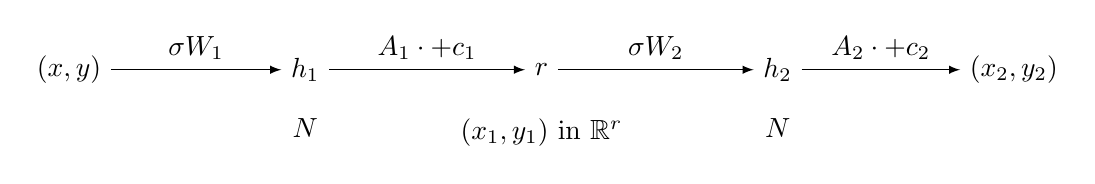
\begin{tikzpicture}
    \node (x) at (0,0) {$(x,y)$}; % input
    \node (h1) at (3,0) {$\bm{h}_1$}; % first wide layer N
    \node (r) at (6,0) {$\bm{r}$}; % bottleneck layer r
    \node (h2) at (9,0) {$\bm{h}_2$}; % second wide layer N
    \node (y) at (12,0) {$(x_2,y_2)$}; % output
    
    \draw[-latex] (x) -- node[above] {$\sigma W_1$} (h1);
    \draw[-latex] (h1) -- node[above] {$A_1 \cdot+c_1$} (r);
    \draw[-latex] (r) -- node[above] {$\sigma W_2$ } (h2);
    \draw[-latex] (h2) -- node[above] {$A_2 \cdot +c_2$} (y);
    
    \node[below] at (3,-0.5) {$N$};
    \node[below] at (6,-0.5) {$(x_1,y_1)$ in $\mathbb{R}^r$};
    \node[below] at (9,-0.5) {$N$};
\end{tikzpicture}
\end{center}
And here N grow to infinity, and r is fixed.

Then the NTK random kernel is:
\begin{equation}
    \Theta^{(\ell)}(x, x') = \Theta^{(\ell-1)}(x, x') \cdot \left(\sigma_A^2\dot{\Sigma}^{(\ell)}(x, x')\right) + \Sigma^{(\ell)}(x, x') +1
\end{equation}

For $\ell=2$, starting from $\Theta^{(0)} = 0$, we have:

\begin{align*}
    \Theta^{(1)} &= \mathbb{E}_{\bm{w}, b} \left[ \sigma(\bm{w}^\top x + \beta b) \sigma(\bm{w}^\top x' + \beta b) \right] + 1 \\
    \Theta^{(2)} &= \Theta^{(1)} \cdot \left(\sigma_A^2 \mathbb{E}_{\bm{w}, b} \left[ \dot{\sigma}(\bm{w}^\top \bm{h}^{(1)}(x) + \beta b) \dot{\sigma}(\bm{w}^\top \bm{h}^{(1)}(x') + \beta b) \bm{w}^\top\bm{w} \right]\right) \\
    &\quad + \mathbb{E}_{\bm{w}, b} \left[ \sigma(\bm{w}^\top \bm{h}^{(1)}(x) + \beta b) \sigma(\bm{w}^\top \bm{h}^{(1)}(x') + \beta b) \right] + 1
\end{align*}

Here, $\Theta^{(1)}$ is a deterministic NNGP kernel (Gaussian Process) since it depends only on the input $x$, while $\Theta^{(2)}$ is a random field (Deep Gaussian Process) that depends on the realization of the first layer's output $\bm{h}^{(1)}$. When $\beta = 0$, these expectations simplify by removing the bias terms $b$. This non-Gaussian nature of the kernels for $\ell > 1$ is a key distinguishing feature of MMNNs compared to standard neural networks.

\newline
When $\beta = 0$, the equations simplify to:
\begin{tcolorbox}[title=Main focus: NTK kernels with $\beta=0$]
\begin{align*}
    \Theta^{(1)} &= \mathbb{E}_{\bm{w}} \left[ \sigma(\bm{w}^\top x) \sigma(\bm{w}^\top x') \right] + 1 \\
    \Theta^{(2)} &= \Theta^{(1)} \cdot \left(\sigma_A^2 \mathbb{E}_{\bm{w}} \left[ \dot{\sigma}(\bm{w}^\top \bm{h}^{(1)}(x)) \dot{\sigma}(\bm{w}^\top \bm{h}^{(1)}(x')) \bm{w}^\top\bm{w} \right]\right) \\
    &\quad + \mathbb{E}_{\bm{w}} \left[ \sigma(\bm{w}^\top \bm{h}^{(1)}(x)) \sigma(\bm{w}^\top \bm{h}^{(1)}(x')) \right] + 1
\end{align*}
\end{tcolorbox}

Note that for stable signal propagation at the Edge of Chaos (EOC), we require for 1 rank hidden layer:
\begin{equation*}
    \sigma_A^2 \cdot \text{Tr}(\Sigma_w) = 2
\end{equation*}

Then for a rank r
\begin{equation*}
    \sigma_A^2 \cdot \text{Tr}(\Sigma_w) = \frac{2}{r}
\end{equation*}

And we assume at least isotropic gaussian for the weights without loss of generality and to ensure fast computations.

This condition ensures the signal neither vanishes nor explodes as it propagates through the network layers.
This also means we need to normalize by $\sqrt{r}$ the output of the first MMNN layer.
We call $x_1$ and $y_1$ the outputs of the first layer unnormalized.

We recall also that $\Sigma^{(1)}$ is the arccosine kernel, which has a closed form in function of the correlation $\rho$ between $x$ and $x'$:
\[
\Sigma^{(1)}(\rho) =  \frac{1}{\pi}\left(\sqrt{1-\rho^2} + \rho(1-\arccos(\rho))\right)
\]

We recall also that $\dot{\Theta}^{(1)}(\rho) = \mathbb{E}_{\bm{w}} \left[  \bm{w}^\top \bm{w} \dot{\sigma}(\bm{w}^\top x) \dot{\sigma}(\bm{w}^\top x') \right]$. We can compute this exactly when $\bm{w}$ is isotropic gaussian with variance 1:




In fact a simple computation takes the expectation of the product of the two derivatives of the ReLU, by independence of $\|\bm{w}\|^2$ and $\mathbb{1}_{\bm{w}^\top x > 0} \cdot \mathbb{1}_{\bm{w}^\top x' > 0}$:
\begin{align*}
\dot{\Theta}^{(1)}(\rho) &= \mathbb{E}_{\bm{w}} \left[  \bm{w}^\top \bm{w} \dot{\sigma}(\bm{w}^\top x) \dot{\sigma}(\bm{w}^\top x') \right] \\
&= \mathbb{E}_{\bm{w}} \left[  \bm{w}^\top \bm{w} \cdot \mathbb{1}_{\bm{w}^\top x > 0} \cdot \mathbb{1}_{\bm{w}^\top x' > 0} \right] \\
&= \mathbb{E}\!\left[ \|\bm{w}\|^2 \right] \cdot \mathbb{P}(\bm{w}^\top x > 0, \bm{w}^\top x' > 0) \\
&= \operatorname{Tr}(\Sigma_w)\left(\frac{1}{2} - \frac{\arccos(\rho)}{2\pi}\right)
\end{align*}
It is just a reformulation of the fact that we integrate over a cone of angle $\arccos(\rho)$ a radial function.

We then write $\Theta^{(2)}$ as a function of $\rho$ and $\rho_1$:
\begin{center}
\boxed{
\begin{aligned}
\Theta^{(2)}(\rho, \rho_1) &= \Theta^{(1)}(\rho) \cdot \sigma_A^2 \operatorname{Tr}(\Sigma_w)  \left(\frac{1}{2} - \frac{\arccos(\rho)}{2\pi}\right) + \frac{1}{r} \cdot \Sigma^{(1)}(\rho_1)\|x_1\| \|y_1\|  + 1 \\[1em]
\text{with} \quad \Sigma^{(1)}(\rho) &=  \frac{1}{\pi}\left(\sqrt{1-\rho^2} + \rho(1-\arccos(\rho))\right)
\end{aligned}
}
\end{center}

where $\rho_1$ is the correlation between the outputs of the first layer, that is a random variable and $\rho$ is the correlation between the inputs.

Note that this multiplicative value is between $0$ and $1$, that is we can compute a lot of stuff after concatenating layers and getting some exponential scaling laws.
We emphasize the fact we multiply by $\|x_1\| \|y_1\|$ which is a random variable, but as we will see, it is independent of the correlation $\rho_1$.

\subsection{Expression for random variables $\rho_1$, $\|x_1\|^2$, $\|y_1\|^2$}
The output of the 1st layer is a gaussian process of dimension r, where each coordinate is a gaussian process with covariance matrix:
\[
\Sigma^{(1)}_i = \mathbb{E}_{\bm{w}} \left[ \sigma(\bm{w}^\top x) \sigma(\bm{w}^\top x') \right]
\]
and the coordinates are $\rho$-correlated. If we stack horizontally the outputs $x_1$ and $y_1$ in a vector of dimension $2r$, the full $2r \times 2r$ covariance matrix is therefore:
\[
\Sigma^{(1)} = \begin{pmatrix}
I & \rho I \\
\rho I & I
\end{pmatrix}
\]
It's a kronecker product of $r$ matrices $I$ and 2d $\rho$ correlated gaussian variables.


it happens, by a magic, that we can compute exactly the joint distribution of the random variable $(\rho_1, \|x_1\|^2, \|y_1\|^2)$ :

\[
\rho_1 = \frac{\sum_{i=1}^r x_i y_i }{\sqrt{\sum_{i=1}^r x_i^2} \sqrt{\sum_{i=1}^r y_i^2}}
\]
The squared norms $x_1^2$ and $y_1^2$ follow a bivariate Kibble distribution and their cosine distance follows an independent Fisher like distribution. The Kibble distribution is defined for $u,v \geq 0$ and $\rho \in [-1,1]$, while the Fisher distribution is defined for $\theta \in [-1,1]$ and $\rho \in [-1,1]$ with $r > 2$.

\begin{align*}
    (\|x_1\|^2, \|y_1\|^2) &\sim \text{Kibble}(r, \rho) \\
    &= \frac{(uv)^{\frac{r/2-1}{2}} e^{-\frac{u+v}{2(1-\rho^2)}}}{\Gamma(r/2) (2(1-\rho^2))^{r/2+1} \rho^{\frac{r/2-1}{2}}} \cdot I_{r/2-1}\left(\frac{\rho\sqrt{uv}}{1-\rho^2}\right) \\[1em]
    \rho_1 &\sim \text{Fisher}(\rho, r) \\
    &= \frac{(r-2)\Gamma(r-1)(1-\rho^2)^{\frac{r-1}{2}}(1-\theta^2)^{\frac{r-4}{2}}}{\sqrt{2\pi}\Gamma(r-\frac{1}{2})(1-\rho \theta)^{r-\frac{3}{2}}} \times {}_2F_1\left(\frac{1}{2}, \frac{1}{2}; r-\frac{1}{2}; \frac{1+\rho \theta}{2}\right)
\end{align*}

where $u = \|x_1\|^2$, $v = \|y_1\|^2$, $\theta = \cos(x_1,y_1)$, and $I_\alpha$ is the modified Bessel function of the first kind.

and the correlation of x,y: 

where $x_1_i$ and $y_1_i$ are $\rho$-correlated gaussian variables.

We ensure that the reader has understood that the correlation of x,y is independent of the squared norms of x,y !

\subsubsection{Final result}
We can then state the final result: For 2 entries x,y in $\mathbb{R}^d$ and a low rank r hidden layer, the NTK for a 2 hidden layer MMNN is:


\begin{center}
    
    \newline
\boxed{
\begin{aligned}
\Theta^{(2)}(x,y) &= \Theta^{(1)}(\rho) \cdot \left(1 - \frac{\arccos(\rho_1)}{\pi}\right)\frac{1}{r}  + \frac{1}{r}\Sigma^{(1)}(\rho_1)\|x_1\| \|y_1\| + 1 \\[1em]
\text{with} \quad \Sigma^{(1)}(\rho) &= \frac{1}{\pi}\left(\sqrt{1-\rho^2} + \rho(1-\arccos(\rho))\right)
\end{aligned}
}
\end{center}

where the random variables follow:
\begin{itemize}
\item $\rho_1 \sim \text{Fisher}(\rho, r)$ is independent of the norms
\item $(\|x_1\|^2, \|y_1\|^2) \sim \text{Kibble}(r, \rho)$ are chi-squared variables with r degrees of freedom from correlated gaussian variables.
\end{itemize}

\begin{center}

\newpage
\section{Fisher, Kibble distributions and the fake "Curse of Dimensionality"}

\subsection{Distribution of the Correlation Coefficient $r$}
Fisher derived the exact law of $r$ in 1915, representing the cosine between Gaussian vectors of dimension $r$ with correlation $\rho$:

\[
p(r|\rho, r) = \frac{(r-2)\Gamma(r-1)(1-\rho^2)^{\frac{r-1}{2}}(1-r^2)^{\frac{r-4}{2}}}{\sqrt{2\pi}\Gamma(r-\frac{1}{2})(1-\rho r)^{r-\frac{3}{2}}} \times {}_2F_1\left(\frac{1}{2}, \frac{1}{2}; r-\frac{1}{2}; \frac{1+\rho r}{2}\right)
\]
Where $\Gamma$ is the gamma function and ${}_2F_1$ is the hypergeometric function.

For large $r$, Fisher's z-transform gives $z = \text{arctanh}(r) \sim \mathcal{N}\left(\text{arctanh}(\rho) + \frac{\rho}{2(r-1)}, \frac{1}{r-3}\right)$. The variance of $r$ decreases as $O(1/r)$. When $\rho \sim O(1/\sqrt{r})$, geometric noise masks correlation.

\subsection{The Kibble Distribution}
The joint law of correlated chi-squared variables $U=\|X\|^2$ and $V=\|Y\|^2$ follows Kibble's 1941 distribution:

\[
f(u, v) = \frac{(uv)^{\frac{r/2-1}{2}} e^{-\frac{u+v}{2(1-\rho^2)}}}{\Gamma(r/2) (2(1-\rho^2))^{r/2+1} \rho^{\frac{r/2-1}{2}}} \cdot I_{r/2-1}\left(\frac{\rho\sqrt{uv}}{1-\rho^2}\right)
\]
Where $\Gamma$ is the gamma function and $I_\alpha$ is the modified Bessel function of the first kind.

Mean $\E[U] = r$ and variance $\Var(U) = 2r$ grow linearly. $U/r$ converges to $\mathcal{N}(1, 2/r)$ with polynomial concentration.


\subsection{Exact moments and correlation for Kibble variables}

Let $(X_i,Y_i)_{i=1}^r$ be i.i.d. Gaussian pairs with zero mean, unit variances and correlation $\rho$, and define
\[
U=\sum_{i=1}^r X_i^2,\qquad V=\sum_{i=1}^r Y_i^2.
\]
Then $(U,V)$ follows Kibble's bivariate chi-square law with $r$ degrees of freedom and correlation $\rho$. By Isserlis' (Wick's) theorem (or by expanding $\E[(X_i-\rho Y_i)^n (Y_i)^m]$ recursively):
\[
\E[X_i^2]=1,\quad \Var(X_i^2)=2,\quad \E[X_i^2Y_i^2]=1+2\rho^2,\quad \Cov(X_i^2,Y_i^2)=2\rho^2.
\]
Using independence across $i$:
\[
\E[U]=r,\quad \Var(U)=2r,\qquad \E[V]=r,\quad \Var(V)=2r,
\]
\[
\Cov(U,V)=\sum_{i=1}^r \Cov(X_i^2,Y_i^2)=2r\,\rho^2,
\]
\[
\Corr(U,V)=\frac{\Cov(U,V)}{\sqrt{\Var(U)\Var(V)}}=\frac{2r\rho^2}{\sqrt{(2r)(2r)}}=\rho^2,
\]
\[
\E[UV]=\E[U]\E[V]+\Cov(U,V)=r^2+2r\,\rho^2.
\]


\subsection{Product of Square Roots of Kibble Variables}
Let $S=\sqrt{U}\sqrt{V}=\|X\|\|Y\|$. Due to correlation between $U$ and $V$, we cannot directly multiply expectations. Instead, using Cauchy-Schwarz inequality:

\[
\E[S^2] = \E[UV] = \E[U]\E[V] + \Cov(U,V) = r^2 + 2r\rho^2
\]

Therefore:
\[
\E[S] \leq \sqrt{\E[S^2]} = r\sqrt{1 + \frac{2\rho^2}{r}}
\]

The variance can be estimated similarly by expanding $(S - \E[S])^2$ and using correlation terms:

\[
\Var(S) \approx \frac{r}{2}(1 + \rho^2) + O(1)
\]

This suggests $S/r$ approaches a distribution with mean $O(\sqrt{1 + \frac{2\rho^2}{r}})$ and variance of order $O(1/r)$.

\subsection{Independence Properties and Asymptotic Behavior}
The orientation variable $r$ is independent of magnitudes $(U,V)$. For the normalized product $S/r$, we have:

\[
\frac{S}{r} = \frac{\|X\|\|Y\|}{r} \xrightarrow{r \to \infty} 1
\]

This convergence occurs with fluctuations of order $O(1/\sqrt{r})$, showing that in high dimensions, the normalized product concentrates around 1 regardless of the correlation $\rho$.


\end{document}